\lstset {language=C++}

\chapter{VS}

VS maakt het mogelijk om logica op een visuele manier inplaats van textuel te schrijven. Er is minder kennis van de onderliggende werking van computer systemen nodig dan voor tekstueel programmeren [?]. Hierdoor kan er zonder kennis van computers en hun werking al snel mee gewerkt worden door niet programmeurs. 

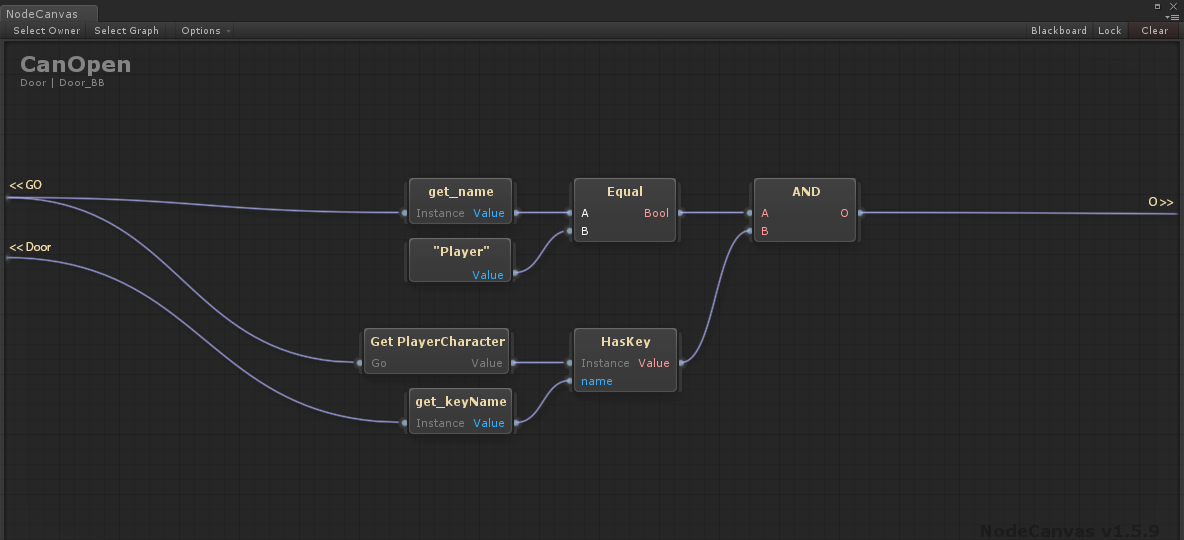
\includegraphics{VisualScriptingExample}

Daarnaast word de mogelijkheden van de visuele programmeer taal ook vaak gelimiteerd om het de gebruiker makkelijker te maken en het programma te beschermen van de gebruiker. Meestal als de limitaties van de visuele scripting taal een probleem worden had de logica beter in een tekstuele taal geschreven kunnen worden.

\section{Use Case's}
Door de jaren heen zijn er voor verschillende doeleinden visuele programmeer talen gemaakt. 
Een aantal voorbeelden zijn

\begin{itemize}  
\item Data flow in applicaties 
\item State flow voor onder andere animaties 
\item Geluids effecten programmeren
\item Gameplay Logica 
\item Programeren leren aan beginners 
\end{itemize}

In deze scriptie word er gefocust op het gebruik van VS voor gameplay logica.

\section{Gameplay Logica}
Het programmeren van gameplay in een spel bestaat voor een groot gedeelte uit de vragen “Wanneer moet iets gebeuren”, “Wat moet er gebeuren” en “Hoe moet dit gebeuren”.
De vragen “Waarom moet iets gebeuren” en “Waar moet dit gebeuren” komen het meeste voor in de gameplay logica van een spel, vaak hebben deze vragen ook een makkelijk antwoord. Helaas zijn deze vragen lastig om te beantwoorden in textuele code.

\subsection{Het afvuren van een projectiel}
Een voorbeeld van deze drie vragen in code is als volgt, voor het voorbeeld laten wij de logica zien van het schieten van een projectiel in c++.

\subsubsection{Tekstuele Implementatie}
In een c++ header bestand registreren wij de volgende functie in onze speler classe.
\begin{lstlisting}
void OnFire();
\end{lstlisting}
Dan tijdens het opzetten van de input voor ons karakter laten we weten wanneer we een projectiel willen schieten.

\begin{lstlisting}
if( EnableTouchscreenMovement(InputComponent) == false )
{
	InputComponent->BindAction(
		"Fire", 
		IE_Pressed, 
		this, 
		&Adpi_unreal_colosseumCharacter::OnFire
	);
}
\end{lstlisting}
Maar omdat de “fire” actie niet werkt op een touch interface moeten we de onfire zelf afvuren als iemand het scherm aanraakt (De logica achter het registeren van touch events word niet getoond maar is wel aanwezig in de speler klasse).

\begin{lstlisting}
void Adpi_unreal_colosseumCharacter::EndTouch(const ETouchIndex::Type FingerIndex, const FVector Location)
{
	if (TouchItem.bIsPressed == false)
	{
		return;
	}
	if( ( FingerIndex == TouchItem.FingerIndex ) && (TouchItem.bMoved == false) )
	{
		OnFire();
	}
	TouchItem.bIsPressed = false;
}
\end{lstlisting}
Vervolgens definiëren we OnFire als volgt

\begin{lstlisting}
void Adpi_unreal_colosseumCharacter::OnFire()
{ 
	// try and fire a projectile
	if (ProjectileClass != NULL)
	{
		const FRotator SpawnRotation = GetControlRotation();
		// MuzzleOffset is in camera space, so transform it to world space before offsetting from the character location to find the final muzzle position
		const FVector SpawnLocation = GetActorLocation() + SpawnRotation.RotateVector(GunOffset);

		UWorld* const World = GetWorld();
		if (World != NULL)
		{
			// spawn the projectile at the muzzle
			World->SpawnActor<Adpi_unreal_colosseumProjectile>(ProjectileClass, SpawnLocation, SpawnRotation);
		}
	}

	// try and play the sound if specified
	...

	// try and play a firing animation if specified
	..
}
\end{lstlisting}
Om de logica te implementeren voor het vuren vuren van de kogel hebben wij nu op vier verschillende plekken de logica moeten verspreiden, hiervan zit de implementatie verspreid in een bestand van 218 regels (zie bijlage standaard playercharcter van Epic).

\subsubsection{Tekstuele Implementatie}
De “Hoe moet dit gebeuren” is een complexe vraag die prima beantwoord word in code. Vooral omdat er verschillende logica achter elkaar plaatsvind, geluid afspelen / animatie starten, en een aantal wiskundige berekeningen. 

Maar de “Wanneer” vraag is makkelijk te beantwoorden. Namelijk als de fire actie uitgevoerd word of als er op het scherm gedrukt word. De logica in blueprints ziet er als volgt uit (in de event graph van een playerCharacter).

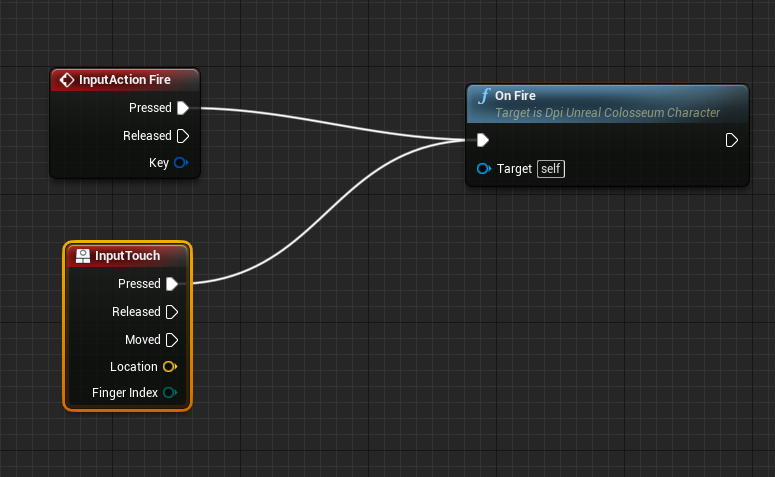
\includegraphics{OnFireBlueprintCall}

In tegenstelling tot de c++ code is de logica van de “Wanneer” vraag dit maal niet verspreid en is het in een oog opslag duidelijk wat er voor zorgt dat er een projectiel geschoten word.